\id{IRSTI 06.75.11}{https://doi.org/10.58805/kazutb.v.1.26-722}

\begin{articleheader}
\sectionwithauthors{A.Zh. Asainov, A.K. Butkenova, K.K. Bokenchin, B.M. Bayadilova, Zh.N. Sadu}{STUDY OF THE PROBLEM OF ENSURING FOOD SECURITY OF THE COUNTRY IN CONDITIONS OF EXTERNAL ENVIRONMENT VOLATILITY}

{\bfseries  
A.Zh. Asainov\authorid,
A.K. Butkenova\textsuperscript{\envelope } \authorid,
K.K. Bokenchin\authorid,
B.M. Bayadilova\authorid,
Zh.N. Sadu\authorid}
\end{articleheader}

\begin{affiliation}
\emph{Kazakh University of Technology and Business named after K. Kulazhanov, Astana, Kazakhstan,}

\raggedright \textsuperscript{\envelope }{\em Correspondent-author: \href{mailto:Butkenova@mail.ru}{\nolinkurl{Butkenova@mail.ru}}}
\end{affiliation}

The article is devoted to the consideration of methodologies for
determining the level of food security, both at the global and regional
levels. The article presents the developments of the
world' s largest \\organizations engaged in ensuring food
security, both on the world stage and within individual states. The
international experience of determining the level of food security, as
well as indicators of food security is considered. Based on the analysis
of indicators, it was concluded that in many countries the methodologies
are very similar, but there is no single concept that could form the
basis of a unified system and that could unite disparate indicators
together.

As the world population continues to grow, much more effort and
innovation is urgently needed to increase agricultural productivity in a
lean manner, improve the functioning of the global value chain, reduce
food losses and food waste, and ensure that all people suffering from
hunger and malnutrition have access to adequate nutrition. Many members
of the international community are convinced that hunger can be
eliminated in the next generation and are working together to achieve
this goal.

There was a need to increase the productivity of agricultural systems
worldwide and to reduce the generation of agricultural waste.
Restorative agricultural practices must be holistically and
comprehensively implemented and food systems, including both food
production and consumption, must be restorative.

Land, healthy soils, water and plant genetic resources are essential
inputs for food production, and their careful use and sustainable
management is becoming a high priority given their increasing scarcity
in many parts of the world. Increasing the productivity of existing
farmland, including restoring degraded land through regenerative
agriculture practices, will also help to counter the need to clear
forests for agriculture. Maintaining the productivity of drylands can be
helped by judicious exploitation of scarce water resources through
improved irrigation and storage technologies coupled with the
development of new drought tolerant crop varieties.

{\bfseries Keywords:} food security, food independence, system of food
security indicators, food security criteria, system of food security
category indicators.

\begin{articleheader}
{\bfseries ИССЛЕДОВАНИЕ ПРОБЛЕМЫ ОБЕСПЕЧЕНИЯ ПРОДОВОЛЬСТВЕННОЙ БЕЗОПАСНОСТИ СТРАНЫ В УСЛОВИЯХ НЕСТАБИЛЬНОСТИ ВНЕШНЕЙ СРЕДЫ}

{\bfseries
А.Ж. Асаинов,
А.К. Буткенова\textsuperscript{\envelope },
К.К. Бокенчин,
Б.М. Баядилова,
Ж.Н. Саду}
\end{articleheader}

\begin{affiliation}
\emph{Казахский университет технологий и бизнеса им.К.Кулажанова, Астана Казахстан,}

\emph{e-mail: Butkenova@mail.ru}
\end{affiliation}

Статья посвящена рассмотрению методик определения уровня
продовольственной безопасности, как на глобальном, так и на региональном
уровнях. В статье представлены разработки крупнейших мировых
организаций, занимающихся обеспечением продовольственной безопасности
как на мировой арене, так и в рамках отдельных государств. Рассмотрен
международный опыт определения уровня продовольственной безопасности, а
также индикаторы продовольственной безопасности. На основе анализа
показателей сделан вывод, что во многих странах методики очень похожи,
но нет единой концепции, которая могла бы лечь в основу единой системы и
объединить разрозненные показатели воедино.

Поскольку население планеты продолжает расти, необходимо срочно
приложить гораздо больше усилий и инноваций, чтобы бережно повысить
производительность сельского хозяйства, улучшить функционирование
глобальной производственно-сбытовой цепи, сократить потери
продовольствия и пищевые отходы, а также обеспечить всем людям,
страдающим от голода и недоедания, доступ к полноценному питанию. Многие
члены международного сообщества убеждены, что голод может быть
ликвидирован уже в следующем поколении, и совместно работают над
достижением этой цели.

Необходимо повысить производительность сельскохозяйственных систем во
всем мире и сократить образование сельскохозяйственных отходов.
Восстановительные методы ведения сельского хозяйства должны применяться
комплексно и всесторонне, а продовольственные системы, включая как
производство, так и потребление продуктов питания, должны быть
восстановительными.

Земля, здоровые почвы, вода и генетические ресурсы растений являются
важнейшими факторами производства продовольствия, и их бережное
использование и устойчивое управление становятся первоочередной задачей,
учитывая их растущую нехватку во многих частях мира. Повышение
продуктивности существующих сельскохозяйственных угодий, включая
восстановление деградировавших земель с помощью методов регенеративного
сельского хозяйства, также поможет противостоять необходимости вырубки
лесов для нужд сельского хозяйства. Поддержанию продуктивности
засушливых земель может способствовать разумная эксплуатация скудных
водных ресурсов путем совершенствования технологий орошения и хранения
воды в сочетании с выведением новых засухоустойчивых сортов
сельскохозяйственных культур.

{\bfseries Ключевые слова:} продовольственная безопасность,
продовольственная независимость, система показателей продовольственной
безопасности, критерии продовольственной безопасности, система
показателей категории продовольственной безопасности.

\begin{articleheader}
{\bfseries СЫРТҚЫ ОРТАНЫҢ ТҰРАҚСЫЗДЫҒЫ ЖАҒДАЙЫНДА ЕЛДІҢ АЗЫҚ ТҮЛІК ҚАУІПСІЗДІГІН ҚАМТАМАСЫЗ ЕТУ ПРОБЛЕМАСЫН ЗЕРТТЕУ}

{\bfseries
А.Ж. Асаинов,
А.К. Буткенова\textsuperscript{\envelope },
К.К. Бокенчин,
Б.М. Баядилова,
Ж.Н. Саду}
\end{articleheader}

\begin{affiliation}
\emph{Қ.Құлажанов атындағы технология және бизнес университеті, Астана, Қазақстан,}

\emph{e-mail:Butkenova@mail.ru}
\end{affiliation}

Мақала жаһандық деңгейде де, аймақтық деңгейде де азық-түлік
қауіпсіздігі деңгейін анықтау әдістерін қарастыруға арналған. Мақалада
әлемдік аренада да, жекелеген мемлекеттер шеңберінде де азық-түлік
қауіпсіздігін қамтамасыз етумен айналысатын ірі әлемдік ұйымдардың
әзірлемелері ұсынылған. Азық-түлік қауіпсіздігі деңгейін анықтаудың
халықаралық тәжірибесі, сондай-ақ азық-түлік қауіпсіздігі индикаторлары
қарастырылды. Көрсеткіштерді талдау негізінде көптеген елдерде әдістер
өте ұқсас, бірақ біртұтас жүйенің негізін құрайтын және әртүрлі
көрсеткіштерді біріктіретін Бірыңғай тұжырымдама жоқ деген қорытындыға
келді.

Планета халқы өсіп келе жатқандықтан, ауыл шаруашылығының өнімділігін
Мұқият арттыру, жаһандық өндіріс және сату тізбегінің жұмысын жақсарту,
азық-түлік шығындары мен азық-түлік қалдықтарын азайту, сондай-ақ аштық
пен тамақтанбаудан зардап шегетін барлық адамдарға толық тамақтануға қол
жеткізу үшін шұғыл түрде көп күш пен инновация қажет. Халықаралық
қоғамдастықтың көптеген мүшелері аштықты келесі ұрпақта жоюға болатынына
сенімді және осы мақсатқа жету үшін бірлесіп жұмыс істейді.

Дүние жүзіндегі ауыл шаруашылығы жүйелерінің өнімділігін арттыру және
ауыл шаруашылығы қалдықтарының түзілуін қысқарту қажет. Ауыл
шаруашылығын қалпына келтіру әдістері жан-жақты және жан-жақты
қолданылуы керек, ал азық-түлік жүйелері, соның ішінде азық-түлік
өндірісі де, тұтыну да қалпына келтірілуі керек.

Жер, сау топырақ, су және өсімдіктердің генетикалық ресурстары
азық-түлік өндірісінің маңызды факторлары болып табылады және оларды
ұқыпты пайдалану және тұрақты басқару әлемнің көптеген бөліктерінде
олардың жетіспеушілігін ескере отырып, бірінші кезектегі міндет болып
табылады. Қолданыстағы ауылшаруашылық жерлерінің өнімділігін арттыру,
соның ішінде регенеративті ауыл шаруашылығы әдістері арқылы деградацияға
ұшыраған жерлерді қалпына келтіру де ауыл шаруашылығының қажеттіліктері
үшін ормандарды кесу қажеттілігіне қарсы тұруға көмектеседі. Құрғақ
жерлердің өнімділігін сақтауға дақылдардың құрғақшылыққа төзімді жаңа
сорттарын өсірумен бірге суару және суды сақтау технологияларын
жетілдіру арқылы тапшы су ресурстарын ұтымды пайдалану ықпал етуі
мүмкін.

{\bfseries Түйін сөздер:} азық-түлік қауіпсіздігі, азық-түлік тәуелсіздігі,
азық-түлік қауіпсіздігі көрсеткіштері жүйесі, азық-түлік қауіпсіздігі
критерийлері, азық-түлік қауіпсіздігі санаты көрсеткіштері жүйесі.

\begin{multicols}{2}
{\bfseries Introduction.} The term «food security» was first introduced
into international circulation after the grain crisis of 1972-1973. The
UN General Assembly in 1974 adopted a resolution «International
Obligations to Ensure Food Security in the World». In this case, world
food security was understood mainly as «maintaining stability in the
markets of food products with the availability of basic foodstuffs for
all countries of the world» {[}1, 2{]}. However, a single categorical
apparatus was not developed at that time. The main activities were
recognized as follows: creation of food reserves at the level of
individual states; organization of monitoring and early warning of food
shortages; provision of food aid to countries in need; involvement of
developing countries in international trade in agricultural products and
food products. A combination of imports and assistance from developed
countries was seen as a means of solving the food problem of most
countries.

In the subsequent period, the world food problem has only worsened.
Annual increase in the world population, reduction and degradation of
cultivated areas, growth of world prices for raw materials and
foodstuffs due to the world crop failure in the countries-exporters of
agricultural products, depletion of natural resources, deterioration of
ecological situation - these and other factors began to hinder further
development of world production of food products and agricultural raw
materials. The quantitative side of the problem did not become
fundamental (according to estimates of the International Food and
Agriculture Organization of the United Nations - FAO, the world is able
to feed 2 times more people living on Earth), because at this time the
differences in the provision of countries with food, inequality
increased. Under the influence of these processes, a new approach to the
problem of food security emerged, according to which the achievement of
food security on a global scale became possible only through ensuring
the latter in each individual state {[}3, 4{]}. In connection with the
new approach to solving the food problem, special attention began to be
paid to food security programs and improving nutrition on the ground.

According to the UN, the COVID-19 pandemic, widespread supply chain
disruptions, climate crisis and extreme weather have resulted in 193
million people in need of emergency assistance losing access to food
security. Globally, the food security situation is worsening. Humanity
is failing to meet the UN hunger elimination targets: 828 million people
- the number of hungry and malnourished people in the world in 2022. EDB
analysts expect a prolonged period of high food prices as a result of
population growth and increased consumption in rapidly developing
countries, as well as under pressure from the adverse effects of climate
change, high prices for energy and its derivatives (including
fertilizers), shortage of skilled labor and new agricultural land.
Against this backdrop, reduced food availability increases the value of
food resources.

Eradicating hunger and malnutrition is one of the greatest challenges
facing humankind. A person is considered «food secure» when he or she
has physical, social and economic access to adequate, safe and
nutritious food that meets his or her dietary needs and food preferences
for an active and healthy life (as defined by the UN Committee on World
Food Security). Urgent action is needed to address global food security
as recognized in the UN Sustainable Development Goals (SDGs). The UN
Secretary-General launched the Zero Hunger program in 2012 during the
Rio+20 World Conference on Sustainable Development . Zero Hunger was
launched to inspire a global movement for a world free of hunger within
a generation.

In 2021, UN Secretary-General António Guterres convened a Summit on Food
Systems as part of the Decade of Action to achieve the 2030 Sustainable
Development Goals (SDGs). The Summit launched bold new actions to make
progress on all 17 SDGs, all of which depend to some extent on
healthier, more resilient and more equitable food systems. Guided by
five action lines, the Summit brought together key players from the
worlds of science, business, politics, health and academia, as well as
farmers, indigenous people, youth organizations, consumer groups,
environmental activists and other key stakeholders. The SDGs set targets
to eradicate hunger, achieve food security, improve nutrition and
develop sustainable agriculture by 2030. These are critical challenges
for the world, requiring international cooperation and policy reform.

While progress has been made in improving food security over the years,
the pandemic has reversed many of these gains, which were already uneven
across countries and regions. The UN Food and Agriculture Organization
estimates that COVID-19 has led to a dramatic increase in malnutrition
among populations. Per capita food availability is projected to increase
by 4\% by 2030, but achieving the zero hunger SDGs will be a challenge.
Uneven growth in food availability across regions will result in
consumers in middle-income countries increasing their food consumption
most significantly, while diets in low-income countries will remain
largely unchanged. This has serious implications for undernourished and
severely food insecure populations who need it most.

{\bfseries Materials and methods.} The article uses methodological tools,
including system analysis, correlation and regression analysis,
summaries and groupings, analysis of empirical distribution series,
multivariate classification, time series analysis and forecasting,
graphical and tabular methods of analysis. The materials for the study
were the analysis of domestic and foreign literature devoted to the
study of food security.

{\bfseries Results and discussions.} The problem of food security has
attracted the attention of the world community since the 70s of the XX
century, when the deficit of the world' s food resources
was revealed. This problem is global in nature: production, distribution
and trade of foodstuffs concern every state regardless of whether its
population suffers from hunger and malnutrition or is provided with
foodstuffs in sufficient or excessive quantities. The reason for its
relevance can be explained in the words of A. Brije-Savarin: «The fate
of nations depends on how they eat».

Food security is a flexible concept and is usually applied at three
levels of aggregation: national, regional, household or individual,
Figure 1.
\end{multicols}

{\bfseries Fig. 1 - Food security}

\begin{multicols}{2}
Food safety is recognized as a priority area of research at the
international level. In February 2001, the World Health Organization
(WHO) held a strategic meeting on food safety planning in Geneva to
discuss the development of the Global Food Safety Strategy {[}5,6{]}.
The international organization Codex Alimentarius deals with the
problems of quality, food safety and standards for components of goods.
The standards developed by this organization are fundamental for the
countries-participants of the General Agreement on Tariffs and Trade
(GATT), if they do not have the ability to scientifically confirm a
higher level of protection of goods.

Thus, food security is a state of a country' s economy in
which a stable supply of agricultural raw materials for the processing
industry and sufficient safe and nutritious food for the population,
taking into account their incomes, as well as relative independence from
imports of raw materials and food, are guaranteed.

Food is at the heart of the Sustainable Development Goals (SDGs), the
UN' s development agenda for the 21st century. The second
of the 17 UN Sustainable Development Goals is «End hunger, achieve food
security and improved nutrition and promote sustainable agriculture».
Achieving this goal by 2030 will require profound changes in the global
food and agriculture system. Some of the components of this goal are:

- ending hunger and ensuring that all people have access to safe and
nutritious food;

- ending all forms of malnutrition;

- doubling agricultural productivity and incomes of small-scale food
producers;

- ensuring sustainable food production systems;

- increasing investment in agriculture;

- correcting and preventing trade restrictions and distortions in world
agricultural markets;

- taking measures to ensure the proper functioning of food commodity
markets.

At the current stage of development, the meaning of the concept of food
security has significantly expanded (compared to the first version of
1996) {[}5, 6{]}. In 2009, the World Food Summit gave a comparative
concept of food security: «Food security exists when all people, at all
times, have physical and economic access to sufficient, safe and
nutritious food to meet their dietary needs and food preferences for an
active and healthy life», and after 2009, food security began to be
understood not only as physical and economic access to food, but also as
social. Based on this definition, food security is based on four main
dimensions, presented in Figure 2.
\end{multicols}

\begin{figure}[H]
	\centering
	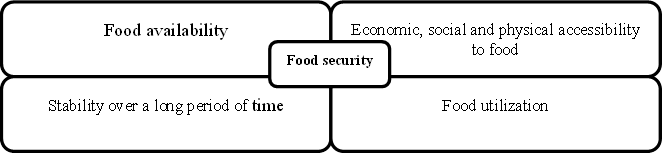
\includegraphics[width=0.6\textwidth]{media/ekon3/image2}
	\caption*{Fig. 2 - The concept of food security based on the four main dimensions}
\end{figure}

\begin{multicols}{2}
In the process of developing the concept of food security, the term
nutritional security was introduced, which was interpreted by the
International Food Policy Research Institute (IFPRI) «as an adequate
level of nutrition in terms of protein, calories, vitamins and minerals
for all household members at all times». In turn, the Food and
Agriculture Organization (FAO - from FAO, Food and Agriculture
Organization) of the United Nations in 2012 proposed the following
definition of nutrition security:

Global food security is maintained by 35 international organizations,
which try to solve not only the above-mentioned problems, but also the
problems of production efficiency, export-import balance, organization
of food aid to the poor population. The world institutional structure of
modern food security began to take its shape and actively formed
immediately after the Second World War, when the enthusiasm of mankind
was filled with the desire to qualitatively change the world for the
better and harmonize it in terms of justice and security. The foundation
of the world food system of food security was the establishment in 1945
under the auspices of the UN Food and Agriculture Organization -- FAO
(Food and Agricultural Organization). Forty-four countries took part in
the creation of a specialized international institution in the field of
nutrition, food and agriculture, which approved the Charter and laid the
foundation for a new milestone in the formation of world food security.

The key international organization dealing with food security is the
Food and Agriculture Organization of the United Nations (FAO). The Food
and Agriculture Organization of the United Nations (FAO) plays an
important role in the management of global world food security,
providing food assistance in 75 countries around the world. FAO, in
accordance with its goals, is called to solve the problem of food
deficit worldwide and its mission «for a world without hunger»
determines its importance in the system of global world economic
regulation of the food sphere.

The current vectors of FAO' s development are in two
directions:

- world food security and access to food for everyone living on the
planet;

- on the basis of innovative achievements of mankind to form high-tech,
sustainable development of food production in balance with social
development of rural areas.

These vectors are aimed at amortization of global challenges of the
modern world:

- uncontrollably rapid growth of the world' s population
with great risks of hunger for the population of poor countries;

- inevitable depletion of the planet' s natural resources
against the background of growing demand for food;

- great competition in the agricultural market, leading to falling
prices and ruin of agricultural producers;

- globalization of the agricultural market and dominance of
transnational corporations in it;

- growing dependence of developing countries on imported products;

- reduction of food consumption in poor countries against the background
of increased consumption in developed countries. To ensure world food
security FAO forms its budget from two sources - mandatory contributions
of participants and voluntary contributions. It is noteworthy that
recently there has been an upward trend in voluntary contributions.

Table 1 compares FAO' s food security assessment
indicators with those used by the U.S. Department of Agriculture.
\end{multicols}

\begin{longtblr}[
  label = none,
  entry = none,
  caption = {\bfseries Table 1 - Food security indicators {[}7, 8{]}},
]{
  colspec = {X[1] X[1]},
  row{1} = {c},
  row{4} = {c},
  row{6} = {c},
  row{8} = {c},
  row{10} = {c},
  row{12} = {c},
  row{14} = {c},
  cell{2}{1} = {c=2}{},
  cell{4}{1} = {c=2}{},
  cell{6}{1} = {c=2}{},
  cell{8}{1} = {c=2}{},
  cell{10}{1} = {c=2}{},
  cell{12}{1} = {c=2}{},
  cell{14}{1} = {c=2}{},
  hlines,
  vlines,
}
U.S. Food Security Indicators                                                                                                                                                                                                                                                                                                                   & FAO Food Security Indicators                                                                                                                                                                                                                                                                                                                                         \\
Availability                                                                                                                                                                                                                                                                                                                                    &                                                                                                                                                                                                                                                                                                                                                                      \\
{Average dietary energy supply\\Average caloric intake\\Share of dietary food, root crops\\and tuber crops\\Average protein content\\Average protein content of animal origin}                                                                                                                                                                  & {Average energy value of the diet\\Average food production\\Share of cereals, root and tuber crops\\in the energy value of the diet\\Average protein intake\\Average animal protein intake}                                                                                                                                                                          \\
Physical access                                                                                                                                                                                                                                                                                                                                 &                                                                                                                                                                                                                                                                                                                                                                      \\
{Percentage of paved roads out of total number of roads\\Railroad density\\Road density}                                                                                                                                                                                                                                                        & {Percentage of paved roads in relation to all roads\\Gross domestic product per capita (purchasing power equivalent)}                                                                                                                                                                                                                                                \\
Economic аccess                                                                                                                                                                                                                                                                                                                                 &                                                                                                                                                                                                                                                                                                                                                                      \\
Index of domestic food price level                                                                                                                                                                                                                                                                                                              & Domestic food industry price index                                                                                                                                                                                                                                                                                                                                   \\
Utilization                                                                                                                                                                                                                                                                                                                                     &                                                                                                                                                                                                                                                                                                                                                                      \\
{Access to improved water resources\\Access to improved treatment services}                                                                                                                                                                                                                                                                     & {Access to improved water sources\\Access to improved sanitation facilities}                                                                                                                                                                                                                                                                                         \\
Outcomes                                                                                                                                                                                                                                                                                                                                        &                                                                                                                                                                                                                                                                                                                                                                      \\
{Inadequate access to food\\Prevalence of undernutrition\\Proportion of expenditure on food by the poor\\Depth of food deficiency\\Prevalence of food inadequacy}                                                                                                                                                                               & {Prevalence of malnutrition\\Share of food expenditures in the budget of poor households\\Extent of food insecurity\\Prevalence of food insecurity}                                                                                                                                                                                                                  \\
Utilization                                                                                                                                                                                                                                                                                                                                     &                                                                                                                                                                                                                                                                                                                                                                      \\
{Proportion of children under 5 years of age with dystrophy\\Proportion of children under 5 years of age with atrophy\\Proportion of children under 5 years of age who weigh less than the normal weight\\Proportion of adults who weigh below the norm}                                                                                        & {Percentage of wasting in children under 5 years of age\\Percentage of children under 5 years of age who are stunted\\Percentage of children under 5 years of age who are underweight\\Percentage of adults who are underweight\\Anemia among pregnant women\\Anemia among children under 5 years of age\\Vitamin A deficiency in the population\\Iodine deficiency} \\
Vulnerability/Stability                                                                                                                                                                                                                                                                                                                         &                                                                                                                                                                                                                                                                                                                                                                      \\
{Domestic food price volatility index\\Variability of food production per capita\\Variability of food supply per capita\\Political stability and absence of\\violence/terrorism\\Volume of imported food in total merchandise exports\\Percentage of arable land equipped with\\Irrigation facilities\\Level of dependence on imported cereals} & {Volatility of domestic food prices\\Variability of food production\\per capita\\Variability of food supply per capita\\Political stability and absence of violence/terrorism\\Share of food imports in total imports of goods\\Percentage of arable land with irrigation equipment\\Degree of dependence on cereal imports}                                         
\end{longtblr}

As can be seen from the table below, both methodologies are quite
similar and there are only differences in some individual items.

\begin{longtblr}[
  label = none,
  entry = none,
  caption = {\bfseries Table 2 - UNICEF indicators for assessing food security and nutrition at national and regional levels {[}9, 10{]}},
]{
  colspec = {X[1.5] X[3] X[7]},
  row{1} = {c},
  cell{2}{1} = {r=5}{c},
  cell{7}{1} = {c},
  cell{8}{1} = {r=7}{c},
  cell{15}{1} = {r=4}{c},
  cell{19}{1} = {r=4}{c},
  cell{23}{1} = {r=3}{c},
  cell{26}{1} = {c},
  cell{27}{1} = {r=7}{c},
  cell{34}{1} = {r=2}{c},
  vlines,
  hline{1-2,7-8,15,19,23,26-27,34,36} = {-}{},
  hline{3-6,9-14,16-18,20-22,24-25,28-33,35} = {2-3}{},
}
{Factors\\taken into account} & Indicator                                                   & Intended for diagnostics                                                                                                                                                                                                                                                                                                                                                                                                                                                                      \\
{nutritional\\status}         & Percentage of body weight deficiency                        & Moderate and severe degree – less than minus two standard deviations from the average weight for a given age among the surveyed population;                                                                                                                                                                                                                                                                                                                                                   \\
                              & Percentage of growth deficit                                & Moderate and severe degree – less than minus two standard deviations from the average height for age among the surveyed population                                                                                                                                                                                                                                                                                                                                                            \\
                              & Percentage of hypotrophy                                    & Moderate and severe degree – less than minus two standard deviations from the average weight for height among the surveyed population                                                                                                                                                                                                                                                                                                                                                         \\
                              & Vitamin A deficiency                                        & The percentage of children aged 6 to 59 months who received at least one capsule of high-dose vitamin A in a given year                                                                                                                                                                                                                                                                                                                                                                       \\
                              & Percentage of mothers with a low body mass index (BMI)      & The percentage of women whose BMI is less than 18.5, where BMI is an indicator of an adult's nutritional status.                                                                                                                                                                                                                                                                                                                                                                              \\
food ration                   & Calorie consumption                                         & Average daily calorie intake – if possible, detailed by age, gender and stage of life cycle                                                                                                                                                                                                                                                                                                                                                                                                   \\
{Health\\status}              & Low birth weight                                            & Percentage of newborns with a body weight of less than 2,500 g                                                                                                                                                                                                                                                                                                                                                                                                                                \\
                              & Under-five mortality                                        & The probability of death from the moment of birth to 5 years per 1,000 live births                                                                                                                                                                                                                                                                                                                                                                                                            \\
                              & rate Infant mortality                                       & Probability of death from birth to 1 year per 1,000 live births                                                                                                                                                                                                                                                                                                                                                                                                                               \\
                              & The prevalence of common diseases                           & Incidence of diarrhea 5 per 1,000: number of children with diarrhea per 1,000 among the surveyed population.                                                                                                                                                                                                                                                                                                                                                                                  \\
                              & Vaccination rate                                            & Percentage of surviving children aged 12-23 months who received the measles vaccine (line A), three DPT vaccinations (DPT) (line B), all vaccinations, namely BCG, three DPT vaccinations, oral polio vaccine, measles vaccine (line C); children who were not vaccinated (line D).                                                                                                                                                                                                           \\
                              & The prevalence of HIV/AIDS in the adult population          & The percentage of the adult population (15-49 years old) living with HIV/AIDS.                                                                                                                                                                                                                                                                                                                                                                                                                \\
                              & Estimated number of people living with HIV/AIDS             & Estimated number of adults and children living with HIV/AIDS                                                                                                                                                                                                                                                                                                                                                                                                                                  \\
                              & HIV prevalence among pregnant women                         & Percentage of blood samples taken from pregnant women aged 14-24 who tested positive for HIV in unrelated anonymous studies                                                                                                                                                                                                                                                                                                                                                                   \\
                              & Children whose parents died of AIDS                         & Estimated number of children (from 0-14 years old) at the end of the year, one or both of whose parents died of AIDS                                                                                                                                                                                                                                                                                                                                                                          \\
                              & Total Fertility Rate (TFR)                                  & The average number of children born to one woman during her lifetime, according to the average fertility rate in her age group for each age.                                                                                                                                                                                                                                                                                                                                                  \\
                              & Water supply and sanitation                                 & Percentage of household members with drinking water supply. Percentage of household members using latrines or toilets                                                                                                                                                                                                                                                                                                                                                                         \\
Education                     & Adult literacy rate                                         & The percentage of the literate population aged 15 years and above                                                                                                                                                                                                                                                                                                                                                                                                                             \\
                              & The level of education                                      & The percentage of the population in this age group who has received any level of education                                                                                                                                                                                                                                                                                                                                                                                                    \\
                              & Literacy rate                                               & The illiterate part of the population (in \%) is considered to be people aged 20 and above who did not go to school or attended primary school for some time.                                                                                                                                                                                                                                                                                                                                 \\
                              & Net percentage of primary school students / attendance      & Percentage of boys and girls enrolled in primary school according to UNESCO (UNESCO Institute of Statistics) reports                                                                                                                                                                                                                                                                                                                                                                          \\
{Food\\availability}          & Population                                                  & The total number of people. The projected population data is based on various predictive models                                                                                                                                                                                                                                                                                                                                                                                               \\
                              & Annual population growth rate                               & The rate at which the population grows/decreases in a single year, expressed as a percentage of the size of the base population.                                                                                                                                                                                                                                                                                                                                                              \\
                              & Average household size                                      & The average number of people in each household, which is why a household is considered to be a person or a group of people living in a common dwelling (or part of it) at least 4 days a week, and who jointly provide themselves with food and basic necessities – in other words, living together as a family unit.                                                                                                                                                                         \\
                              & Food production                                             & {Climate indicators:\\- amount of precipitation (magnitude, distribution); t temperature (average annual average, temperature range throughout the year); wind; floods, droughts;\\Crop production and production system:\\- the main crop (food, cash); production system, etc.\\Land and soil: soil quality (depletion, desertification); availability/shortage of land\\The main diseases of livestock and crops;\\Methods of production/agriculture/animal husbandry Shortage of workers} \\
Economic indicators           & Food expenses                                               & {- general expenses;\\- food expenses;\\- share of food expenses}                                                                                                                                                                                                                                                                                                                                                                                                                             \\
                              & Infrastructure                                              & {- Availability of roads (km of roads);\\- availability of schools (number of schools/residents);\\- medical care (number of hospital beds, degree of vaccination, etc.);\\- markets (distance to local/regional markets), etc.}                                                                                                                                                                                                                                                              \\
                              & Markets                                                     & {- Types of goods in local/regional markets;\\- Prices for basic food products;\\- Price fluctuations , etc.}                                                                                                                                                                                                                                                                                                                                                                                 \\
                              & Gross national income per capita                            & GNI per capita is the gross national income divided by the average annual population.                                                                                                                                                                                                                                                                                                                                                                                                         \\
                              & GDP per capita                                              & Gross domestic product (GDP) is the amount of value added produced by all resident producers plus any taxes on products (minus subsidies) not included in the cost of products. GDP per capita is the gross domestic product divided by the average annual population.                                                                                                                                                                                                                        \\
                              & Percentage of the population living below the poverty level & The usual method of measuring poverty is based on income or consumption level. A person is considered poor if his level of consumption or income is below a certain minimum level that allows him to meet basic needs.                                                                                                                                                                                                                                                                        \\
                              & Purchasing Power Parity (PPP)                               & Purchasing power parity measures the relative purchasing power in currencies of different countries                                                                                                                                                                                                                                                                                                                                                                                           \\
                              & The Gini coefficient                                        & The Gini coefficient is a measure of income inequality. It is a number from 0 to 1, where 0 means complete equality (all people's income is the same), and 1 means complete inequality (i.e. one person gets all the income, everyone else gets nothing).                                                                                                                                                                                                                                     \\
                              & Social and political environment                            & {- Political stability;\\- migration rate;\\- conflicts/ uprisings}                                                                                                                                                                                                                                                                                                                                                                                                                           
\end{longtblr}

\begin{multicols}{2}
International and national organizations have also developed standards
for per capita food consumption. These indicators have different values
in different countries and in different years. This is due to
peculiarities in the composition and structure of the population by
years, which is reflected in the average values of indicators; with
differences in natural and climatic conditions and traditions of the
population; with changes in scientific data on the structure of
nutrition and the amount of food consumed; other reasons (social,
political, etc.).

In the USA, Japan, most countries of the European Union the issues of
food supply have been generally solved, and the remaining problems are
connected with social, ecological, medical and cultural aspects; whereas
in many developing countries the problem of hunger remains acute, as it
was mentioned above 4, caused by poor development of agrarian
production, poverty, low incomes of the population and military
conflicts.

Food security in Canada, is not as volatile as in other countries and
factors such as inflation and COVID-19 have significantly affected food
security in the country. According to Statistics
Canada' s 2022 report, about 18.4 percent of residents in
10 Canadian provinces face food insecurity. The percentage of households
experiencing food insecurity increased in all provinces -- an increase
from pre-Covid-19 data in 2019.

While Covid-19 has dramatically contributed to worsening food
insecurity, millions of people have already been affected. According to
the Global Food Crisis Report, countries affected by conflict, economic
crisis and climate change are most at risk: the Democratic Republic of
Congo, Ethiopia, Afghanistan, Nigeria, Yemen, Myanmar, Syria, Sudan,
Ukraine and Pakistan are among the top 10 most vulnerable countries.

The PRC leadership has pursued a food security policy since 1978. In
1996, the White Paper on China' s Food Problem was
developed and a red line was set for the country' s food
self-sufficiency at a level of at least 95\% 24; 25. To achieve this
goal, the PRC has adopted a number of legislative acts, medium- and
long-term programs: the Law of the PRC on Agriculture, the Program for
Support and Development of Poor Rural Areas, the Program for Development
of Food Production and Improvement of its Nutritional Quality, the
Program for Development of Agricultural Science and Technology, and
others.

To ensure food security, cooperation between countries within the CIS
can be considered important. The CIS leadership is working to achieve
and maintain food security of its member states. This is considered one
of the priority areas of interstate cooperation and the most important
factor in ensuring national security of the states, is based on the
processes of interstate specialization and integration in the sphere of
agro-industrial complex, the development of exports within the
Commonwealth and the provision of targeted assistance to improve the
nutrition of various segments of the population through the
implementation of programs: «school meals», «summer meals», «food
stamps», «mother and child» nutrition, etc.; unification of legislative
normative and other documents, state quality standards for raw materials
and food products; organization of quality and safety control of
products along the entire technological chain and border control;
stimulation of production of high-quality products and their
certification, etc. The Concept and Complex of Joint Measures to Improve
Food Security of the CIS members have been developed and adopted. They
provide for a fuller and more efficient use of natural, production,
economic and financial resources. To achieve a synergetic effect and
find adequate concessions in solving problems related to agriculture,
water resources, energy, land resources and climate change, it is
necessary to more actively involve decision-making processes on an
integrated basis at the national and regional levels.

{\bfseries Conclusion.} Foreign experience in ensuring food security and
sustainable development of agriculture indicates that increasing the
competitiveness of the relevant branch of the national economy is
impossible without an effective mechanism of state support for
agricultural producers. The systematic study of various aspects of
ensuring long-term sustainability of the food system is of paramount
importance for improving public policy for the development of the
agro-industrial complex of the country and its regions.

There is a need to increase the productivity of agricultural systems
worldwide and to reduce agricultural waste generation. There is a need
to adopt sustainable agricultural practices in a holistic and integrated
manner and to achieve sustainable food systems, including both food
production and consumption.

Ensuring food security requires the development of theoretical
foundations, including precise definitions of the conceptual apparatus
(food security and nutrition security; food independence, etc.),
correlation of terms; allocation of levels and definition of principles
for ensuring food security at different levels of governance, etc. The
theoretical framework should be developed.

For practical realization of theoretical results of scientific research
it is necessary to study the available international and domestic
experience in ensuring food security. Given the global nature of the
modern economy and the basic importance of the problem, it is advisable
to link its solution to the issues of international cooperation in the
field of providing the population with food.

In the coming decades, climate change, global population growth, rising
food prices and environmental stressors will have a significant but
uncertain impact on food security. Humanity faces the need for
adaptation strategies and policy responses to global change, including
options for addressing water allocation, land use patterns, food trade,
post-harvest food processing, and food prices and safety.

Cooperation of the post-Soviet countries within the framework of
international associations will make it possible to confront
international challenges and other risks, ensuring food security of each
state. Ensuring food security of the country, it is necessary to
introduce the latest technologies and move to a digital economy in the
agro-industrial complex, to develop unified high quality requirements
for products within the framework of international organizations (EAEU,
etc.), to establish export and import quotas, ensuring, as a priority,
the food security of their country and allied countries. Income plays an
important role in ensuring food security of the family and each person,
preserving his/her efficiency and health: the level of wages, pensions
and benefits, etc.; which requires attention at all levels of the
management hierarchy.
\end{multicols}

\begin{center}
{\bfseries References}
\end{center}

\begin{references}
1. Global Food Security Index. {[}Electronic resource{]}. - Access mode:
\href{https://foodsecurityindex.eiu.com/Index}{https://foodsecurityindex.eiu.com}. Date of address: 10.09.2024.

2. Finskaja pjaterka: Pereosmyslivaja edu -- ot polja do tarelki.
{[}Jelektronnyj resurs{]}. -- Rezhim dostupa:
\href{https://www.goodnewsfinland.com/ru/feature/finskaya-pyaterka-pereosmyslivaya-edu-ot-polya-do-tarelki}{https://www.goodnewsfinland.com}...
Data obrashhenija: 10.09.2024.{[}in Russian{]}

3. Ob obespechenii prodovol' stvennoj bezopasnosti. Zakon
Respubliki Armenija, 7 maja 2002 g. № ZR-339 // Armenian Legal
Information System. {[}Jelektronnyj resurs{]}. -- Rezhim dostupa:
\href{https://www.arlis.am/DocumentView.aspx?docid=63049}{https://www.arlis.am}. Data
obrashhenija:10.09.2024.{[}in Russian{]}

4. Ob utverzhdenii Koncepcii obespechenija
prodovol' stvennoj bezopasnosti Respubliki Armenija.\\
Rasporjazhenie Prezidenta Respubliki Armenija, 18 maja 2011 g., №
NK-91-N. {[}Jelektronnyj resurs{]}. -- Rezhim dostupa:
\href{http://www.eurasiancommission.org/ru/act/prom\_i\_agroprom/dep\_agroprom/Pages/National-production-plans.aspx}{http://www.eurasiancommission.org}. Data obrashhenija: 15.09.2024. {[}in
Russian{]}

5. O Strategii osnovnyh napravlenij, obespechivajushhih jekonomicheskoe
razvitie sel' skohozjajstvennoj sfery Respubliki Armenija
na 2020-2030 gody. Postanovlenie Pravitel' stva
Respubliki Armenija, 19 dek. 2019 g., № 1886-L. -- {[}Jelektronnyj
resurs{]}. -- Rezhim dostupa: \href{https://www.arlis.am/DocumentView.aspx?DocID=137852}{https://www.arlis.am}. Data obrashhenija: 15.09.2024. {[}in
Russian{]}

6. O Doktrine nacional' noj
prodovol' stvennoj bezopasnosti do 2030 goda Respubliki
Belarus'. \\Postanovlenie Soveta Ministrov Resp.
Belarus', 15 dek. 2017 g., № 962 // Ministerstvo
sel' skogo hozjajstva i prodovol' stvija
Respubliki Belarus'. -- {[}Jelektronnyj resurs{]}. Rezhim
do-stupa: \href{https://mshp.gov.by/documents/plant/dccea377014340f4.html}{https://mshp.gov.by}.
Data obrashhenija: 15.09.2024. {[}in Russian{]}

7. Ob utverzhdenii Doktriny prodovol' stvennoj
bezopasnosti Rossijskoj Federacii {[}Jelektronnyj resurs{]}: Ukaz
Prezidenta Rossijskoj Federacii, 21 janv. 2020 g. № 20 //
Konsul' tant-Pljus. Rossija. -- M., 2020. Data
obrashhenija: 16.09.2024. {[}in Russian{]}

8. O gosudarstvennom regulirovanii razvitija agropromyshlennogo
kompleksa i sel' skih territorij \\{[}Jelektronnyj
resurs{]}: Zakon Respubliki Kazahstan, 8 ijulja 2005 g. № 66 //
Informacionno-pravovaja sistema normativnyh pravovyh aktov Respubliki
Kazahstan IPS «Әdіlet». - Re-zhim dostupa:\\
\href{http://adilet.zan.kz/rus/docs/Z050000066}{http://adilet.zan.kz}. Data obrashhenija: 15.09.2024.
{[}in Russian{]}

9. O nacional' noj bezopasnosti Respubliki Kazahstan
{[}Jelektronnyj resurs{]}: Zakon Respubliki Kazahstan, 6 janvarja 2012
g. № 527-IV // Informacionno-pravovaja sistema normativnyh pravovyh
aktov Respubliki Kazahstan IPS «Әdіlet».- Rezhim dostupa:
\href{https://adilet.zan.kz/rus/docs/Z1200000527}{https://adilet.zan.kz}. Data obrashhenija:
01.10.2024. \\{[}in Russian{]}

10. O prodovol' stvennoj bezopasnosti Kyrgyzskoj
Respubliki {[}Jelektronnyj resurs{]}: Zakon Kyrgyzskoj Respubliki ot 4
avg. 2008 g. № 183 // Centralizovannyj Bank Dannyh Pravovoj In-formacii
Kyrgyzskoj Respubliki. -- Rezhim dostupa:
\href{http://cbd.minjust.gov.kg/act/view/ru-ru/202397?cl=ru-ru}{http://cbd.minjust.gov.kg}. Data
obrashhenija: 01.10.2024. {[}in Russian{]}
\end{references}

\begin{authorinfo}
\emph{{\bfseries Information about the authors}}

Asainov A. Zh.- PhD student at the Higher University of Mongolia, Senior
Lecturer at the Kazakh University of Technology and Business named after
K. Kulazhanov, Astana, Kazakhstan,
\href{mailto:arhat_asainov@mail.ru}{\nolinkurl{arhat\_asainov@mail.ru}};

Butkenova A.K. - Doctor of Science, Associate at the Kazakh University
of Technology and Business named after K. Kulazhanov, Astana,
Kazakhstan,
\href{mailto:Butkenova@mail.ru}{\nolinkurl{Butkenova@mail.ru}};

Bokenchin K.K. - PhD, Associate Professor at the Kazakh University of
Technology and Business named after K. Kulazhanov, Astana, Kazakhstan,
\href{mailto:bokenchin.k@mail.ru}{\nolinkurl{bokenchin.k@mail.ru}};

Bayadilova B.M{\bfseries .-} PhD; Associate Professor Kazakh University of
Technology and Business named after K. Kulazhanov, Astana, Kazakhstan,
e-mail: \href{mailto:melisovna@mail.ru}{\nolinkurl{melisovna@mail.ru}};

Sadu Zh.N.- Ph.D. (Econ.), Senior Lecturer, Kazakh University of
Technology and Business named after K. Kulazhanov, Astana, Kazakhstan,
е-mail: \href{mailto:sdm_2008@mail.ru}{\nolinkurl{sdm\_2008@mail.ru}}

\emph{{\bfseries Сведения об авторах}}

Асаинов А.Ж.- докторант Высшего университета Монголии, старший
преподаватель Казахский университет техноло-гии и бизнеса имени К.
Кулажанова, Астана, Казахстан,
\href{mailto:arhat_asainov@mail.ru}{\nolinkurl{arhat\_asainov@mail.ru}};

Буткенова А.К - доктор по профилю, ассоциированный профессор Казахский
университет технологии и бизнеса имени К. Кулажанова, Астана, Казахстан,
\href{mailto:Butkenova@mail.ru}{\nolinkurl{Butkenova@mail.ru}};

Бокенчин К.К.- доктор PhD, ассоциированный профессор Казахский
университет технологии и бизнеса имени К. Кулажанова, Астана, Казахстан,
\href{mailto:bokenchin.k@mail.ru}{\nolinkurl{bokenchin.k@mail.ru}};

Баядилова Б.М. -доктор Ph.D; ассоциированный профессор Казахский
университет технологии и бизнеса имени К. Кулажанова, Астана, Казахстан,
e-mail: \href{mailto:melisovna@mail.ru}{\nolinkurl{melisovna@mail.ru}};

Саду Ж.Н.- к.э.н, старший преподаватель, Казахский университет
технологии и бизнеса имени К. Кулажанова, Астана, Казахстан, е-mail:
\href{mailto:sdm_2008@mail.ru}{\nolinkurl{sdm\_2008@mail.ru}}
\end{authorinfo}
